
\section{Ubuntu: An open source OS}
\begin{figure}[!ht]
\centering

\includegraphics[width=0.3\textwidth]{input/images/ubuntu.png}                   
\caption{Ubuntu}
\hspace{-1.5em}
\end{figure}
During my training, I also got familiar with a great and open source Operating System, Ubuntu. Firstly, it was quite difficult for a regular MS Windows user to port to Ubuntu. I did all of my project work using this vast operating system. \\
Ubuntu is a Debian-based Linux operating system, with Unity as its default desktop environment. It is based on free software and named after the Southern African philosophy of ubuntu (literally, "human-ness"), which often is translated as "humanity towards others" or "the belief in a universal bond of sharing that connects all humanity".\\
It came under Linux. A kernel normally used by many of the computer persons.You will rarely see a person who is unaware of the term Linux. From perspective of a computer simpleton the one who uses linux mostly shall be having a good knowledge regarding the working of shell,kernel etc.\\

Linux was created by Linus Torvalds. One of a gem of computer scientist who is popular for his OS.\\
Linus was one of the student in Finland and had read a book Operating Systems: Design and Implementation by Andrew S. Tanenbaum.\\
In this book the professor explained about the working of Kernel. To my strange is that he had given the whole source code of his kernel named MINIX in that book. Its really weird but acts as a lucky draw for LInus who took interest in this and with the help of MINIX he created a new OS named Linux. He had told about Andrew in his acknowledgement.\\

Ubuntu's goal is to be secure "out-of-the box". By default user's programs run with low privileges and cannot corrupt the operating system or other user's files. For increased security, the sudo tool is used to assign temporary privileges for performing administrative tasks, which allows the root account to remain locked and helps prevent inexperienced users from inadvertently making catastrophic system changes or opening security holes.\\

\subsection{Installing Ubuntu}
When it comes to installing popular Linux flavour Ubuntu, there are so many useful snippets of information on blogs and guides all over the internet. If you Google “How to install Ubuntu”, you’ll see what I mean.
Here’s how to install Ubuntu:
How To Install Ubuntu Summary
\begin{itemize}
	\item Download Ubuntu
	\item Check if Your Computer will Boot from USB
	\item Make BIOS Changes
	\item Try Ubuntu Before you Install It
	\item Create Bootable USB
	\item Install Ubuntu
	\item Create a username, password, and computer name. You will login with this user id after the installation is complete.
\end{itemize}
For an Ubuntu beginner or curious Windows intermediate user, there’s no single, simple source of information when it comes to getting started. One thing I have noticed is that there’s a lot of technical jargon and sometimes unnecessary terminal commands in lengthy forum posts, but no simple “how to” guides, which I think might put some people off! A shame, when you think about how easy Ubuntu is to install, use and tweak to look really cool!
\subsubsection{Download Ubuntu}
For you first need to download a Ubuntu .ISO CD image file. In this example we install Ubuntu version 15.10. But it does not matter what version you use.
We downloaded Ubuntu using a bittorrent client from here because the file is over 1GB in size. Using torrent lets you resume the download in case there is some interruption. Download it either way you want.
It is important that you download the Desktop version. If you download the Server version it will not install any graphical desktop and you will have to add that manually.
\subsubsection{Try before installing}
If you want to try Ubuntu before installing that you can run it from the USB drive using UnetBootin (Which we use in the next section to create the bootable USB). Also the Ubuntu installation screens will give you that option too.
\subsubsection{Install Ubuntu}
Once you get the bootable USB working follow the screens below to install USB:
\begin{figure}[!ht]
	\centering
	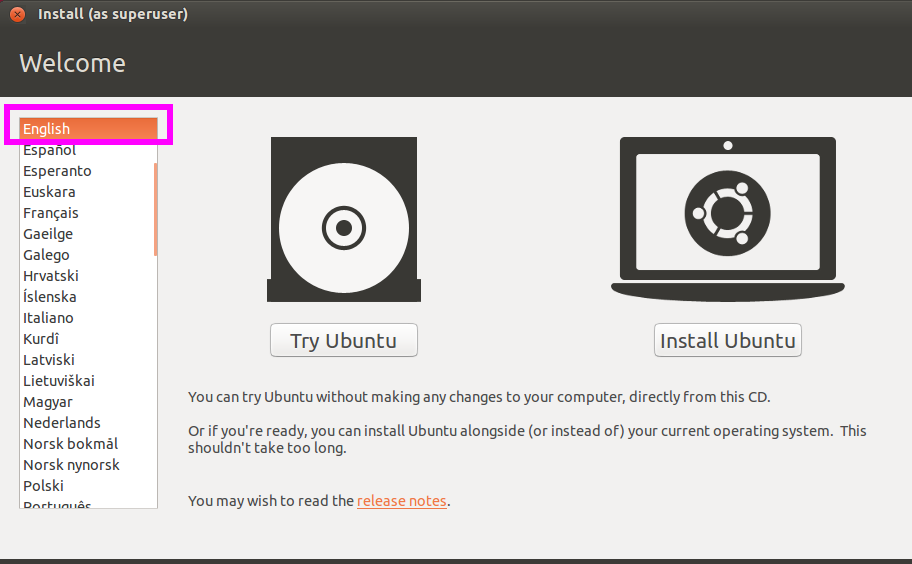
\includegraphics[scale=0.5]{input/images/ubuntu1.png}                   
	\caption{Ubuntu1}
	\hspace{-1.5em}
\end{figure}
\begin{figure}[!ht]
	\centering
	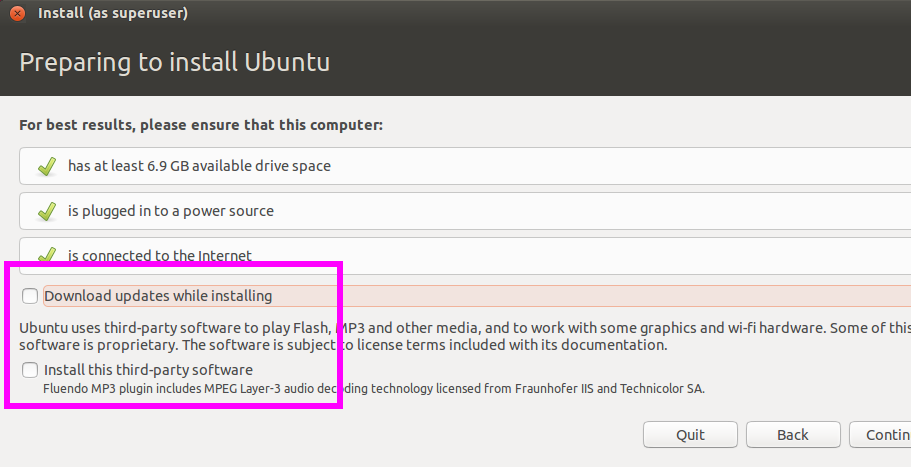
\includegraphics[scale=0.5]{input/images/ub2.png}                   
	\caption{Ubuntu2}
	\hspace{-1.5em}
\end{figure}
\begin{figure}[!ht]
	\centering
	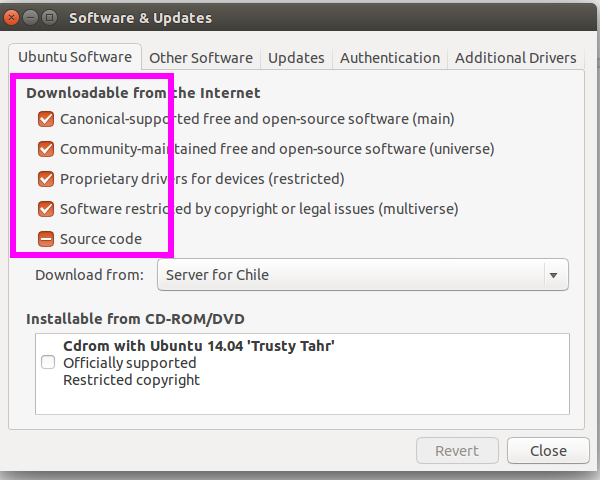
\includegraphics[scale=0.5]{input/images/ub3.png}                   
	\caption{Ubuntu3}
	\hspace{-1.5em}
\end{figure}
\begin{figure}[!ht]
	\centering
	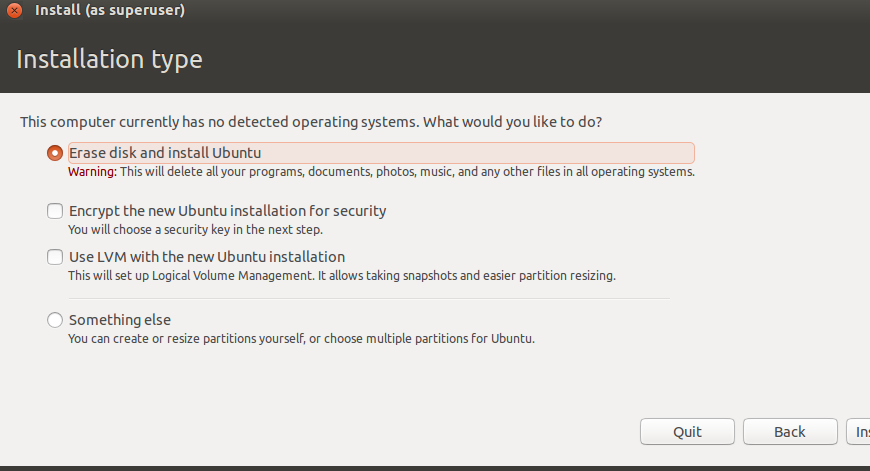
\includegraphics[scale=0.5]{input/images/ub4.png}                   
	\caption{Ubuntu4}
	\hspace{-1.5em}
\end{figure}
\begin{figure}[!ht]
	\centering
	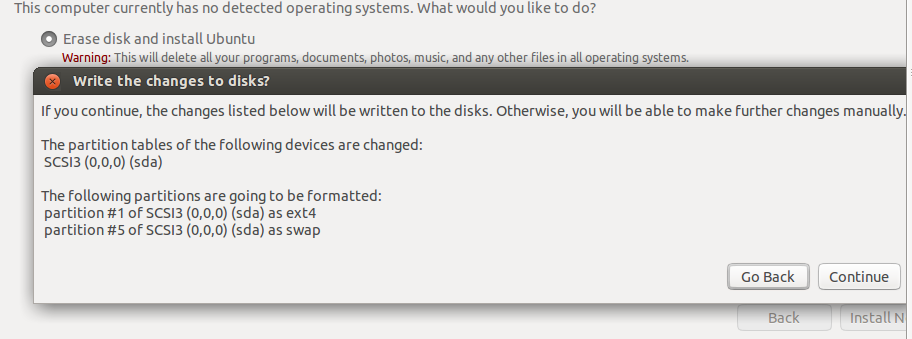
\includegraphics[scale=0.5]{input/images/ub5.png}                   
	\caption{Ubuntu5}
	\hspace{-1.5em}
\end{figure}
\begin{figure}[!ht]
	\centering
	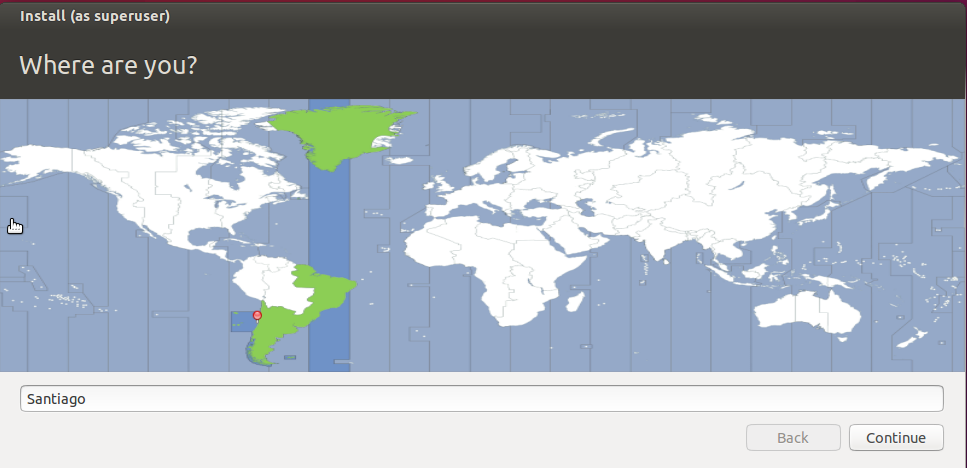
\includegraphics[scale=0.5]{input/images/ub6.png}                   
	\caption{Ubuntu6}
	\hspace{-1.5em}
\end{figure}
\begin{figure}[!ht]
	\centering
	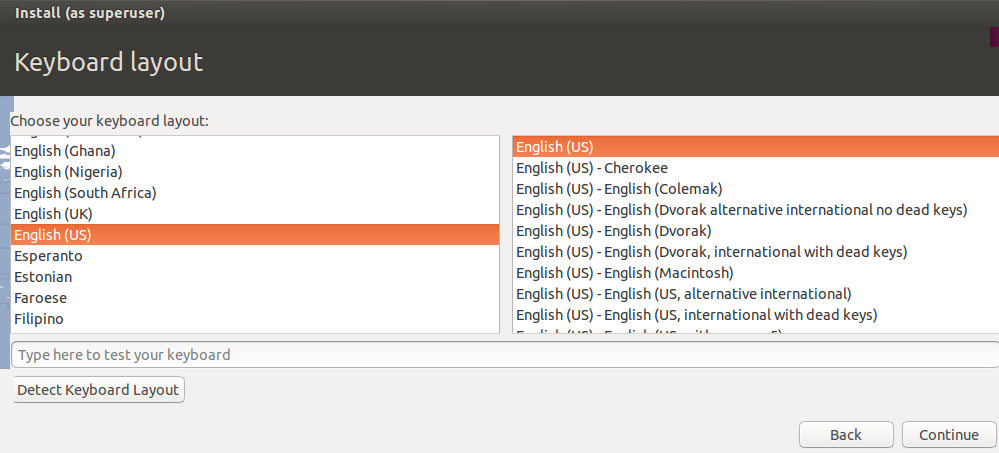
\includegraphics[scale=0.5]{input/images/ub7.png}                   
	\caption{Ubuntu7}
	\hspace{-1.5em}
\end{figure}
\begin{figure}[!ht]
	\centering
	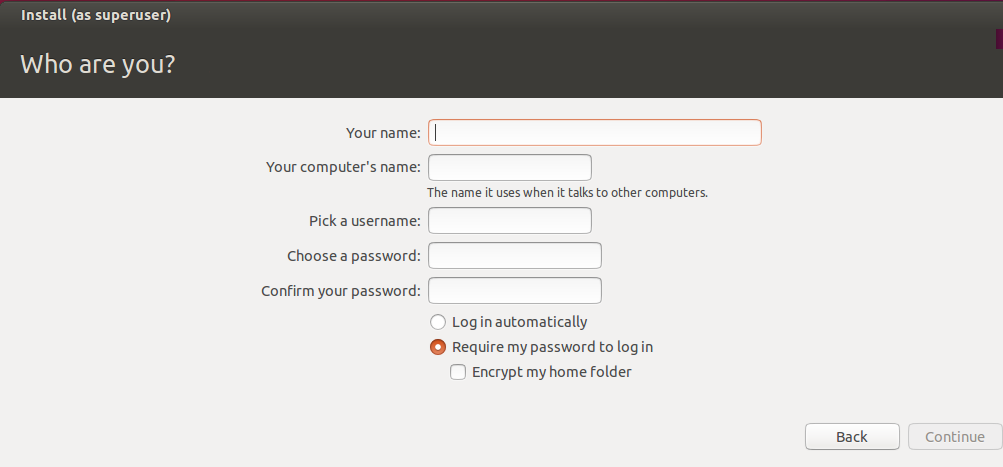
\includegraphics[scale=0.5]{input/images/ub8.png}                   
	\caption{Ubuntu8}
	\hspace{-1.5em}
\end{figure}
\begin{figure}[!ht]
	\centering
	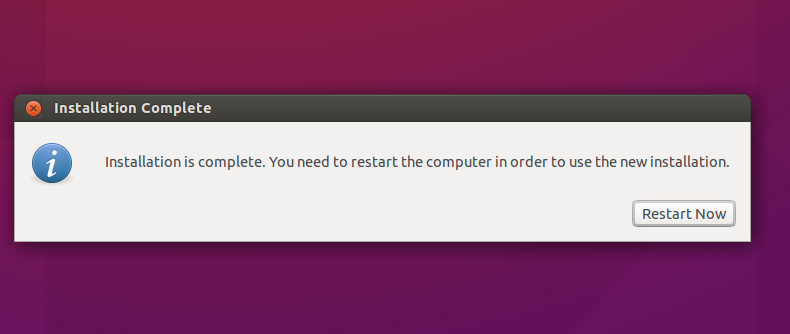
\includegraphics[scale=0.5]{input/images/ub9.png}                   
	\caption{Ubuntu9}
	\hspace{-1.5em}
\end{figure}